\chapter{RMN del protón}\label{ch:g12:proton-nmr}

En un hospital, un paciente está tumbado dentro del anillo de un aparato
de resonancia magnética, y en la pantalla aparece una imagen de los
tejidos blandos del cuerpo, construida a partir de las respuestas de los
\omterm{def:g9:inside-the-atom:nucleus}{núcleos} de hidrógeno de su agua y de sus grasas. En un laboratorio de
química, un pequeño tubo de vidrio con unos miligramos de un compuesto
desciende al interior de un imán potente, y aparece un espectro obtenido
del mismo modo: un imán intenso, una señal de radio y \omterm{def:g9:inside-the-atom:nucleus}{núcleos} de
hidrógeno que le responden. En el espectrómetro del químico, cada \omterm{def:g9:inside-the-atom:nucleus}{núcleo}
de hidrógeno responde de forma un poco distinta según sus vecinos, y el
espectro es un mapa de los \omterm{def:g7:atoms-and-molecules:atom}{átomos} de hidrógeno de la \omterm{def:g7:atoms-and-molecules:molecule}{molécula}.

\begin{recall}
Un \omterm{def:g11:infrared:spectrum}{espectro infrarrojo} muestra qué enlaces contiene una \omterm{def:g7:atoms-and-molecules:molecule}{molécula}
(\cref{ch:g11:infrared}). \omterm{def:g11:functional-groups:functional-group}{Grupos funcionales}, familias e \omterm{def:g11:organic-skeletons:isomer}{isómeros}
(\cref{ch:g11:functional-groups}, \cref{ch:g11:organic-skeletons}).
\end{recall}

\begin{omfigure}
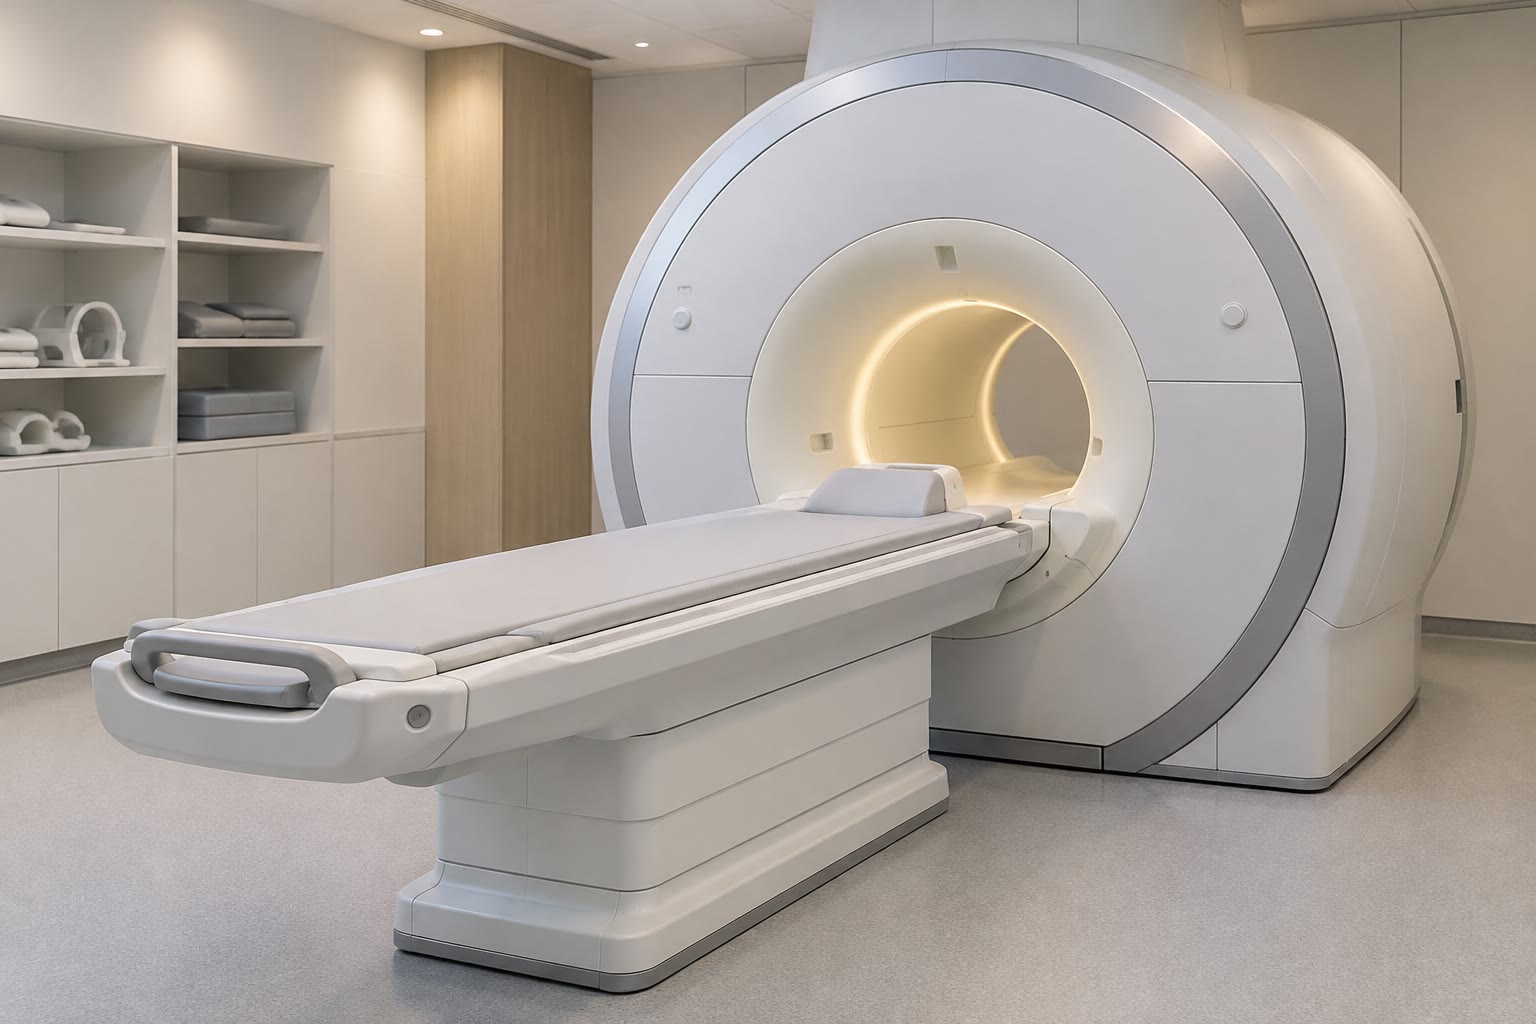
\includegraphics[width=0.48\linewidth]{images/book1/ai/g12-mri-room.jpg}

{\small Un aparato de resonancia magnética: la misma física que la del
espectrómetro de RMN del químico.}
\end{omfigure}

\section{Protones en un campo magnético}

El \omterm{def:g9:inside-the-atom:nucleus}{núcleo} de un \omterm{def:g7:atoms-and-molecules:atom}{átomo} de hidrógeno es un único \omterm{def:g9:inside-the-atom:proton}{protón}. Colocado en un
campo magnético intenso, absorbe ondas de radio de una frecuencia
precisa; el cómo y el porqué pertenecen a la física y no hacen falta aquí.
Lo que importa al químico es que los \omterm{def:g9:inside-the-atom:nucleus}{electrones} que rodean a un \omterm{def:g9:inside-the-atom:proton}{protón} lo
apantallan ligeramente del campo, y que este apantallamiento depende de
los \omterm{def:g7:atoms-and-molecules:atom}{átomos} cercanos: un \omterm{def:g9:inside-the-atom:proton}{protón} vecino de un \omterm{def:g7:atoms-and-molecules:atom}{átomo} de oxígeno
electronegativo, que atrae los \omterm{def:g9:inside-the-atom:nucleus}{electrones}, absorbe a una frecuencia
ligeramente distinta de la de un \omterm{def:g9:inside-the-atom:proton}{protón} de una cadena hidrocarbonada. Las
diferencias son minúsculas, unas millonésimas de la frecuencia, y se
expresan en partes por millón.

\begin{omfigure}
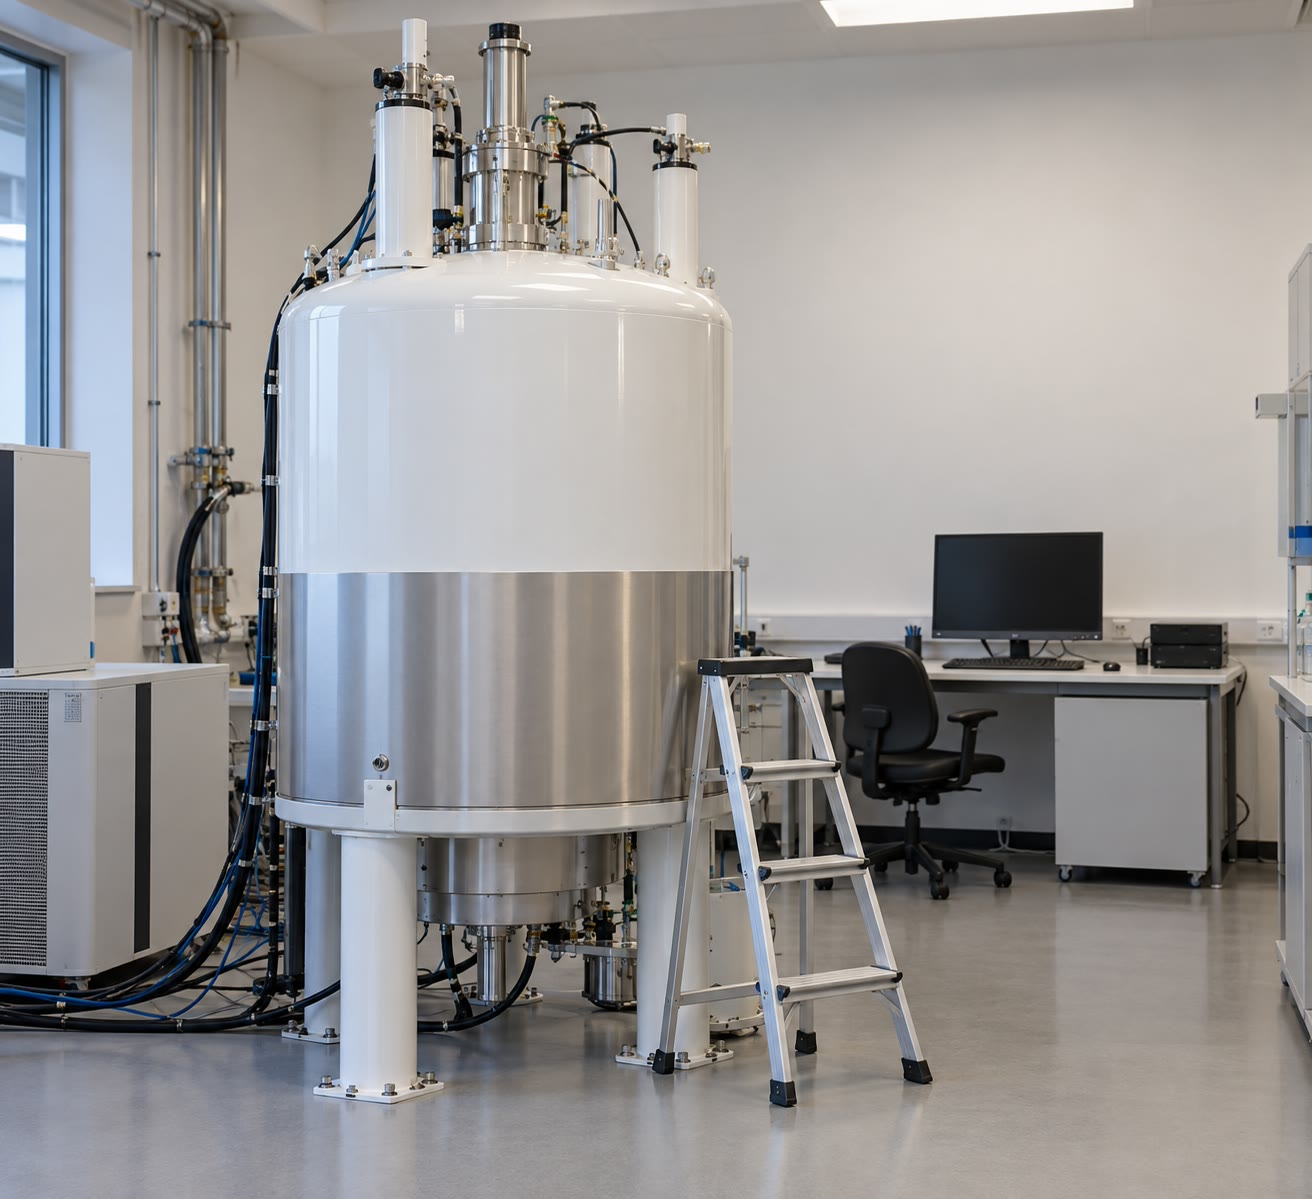
\includegraphics[width=0.42\linewidth]{images/book1/ai/g12-nmr-magnet.jpg}

{\small El imán de un espectrómetro de RMN.}
\end{omfigure}

\begin{definition}[Espectro de RMN, desplazamiento químico]\label{def:g12:proton-nmr:spectrum}
Un \emph{espectro de RMN}\index{espectro de RMN} del \omterm{def:g9:inside-the-atom:proton}{protón} (resonancia
magnética nuclear) muestra las señales absorbidas por los \omterm{def:g9:inside-the-atom:nucleus}{núcleos} de
hidrógeno de un compuesto. La posición de una señal es su
\emph{desplazamiento químico}\index{desplazamiento quimico@desplazamiento químico} $\delta$, en partes por millón (\si{ppm}),
medido a partir de la señal de un compuesto de referencia, el tetrametilsilano
\ce{Si(CH3)4} (TMS), fijada en $\delta = 0$. El eje de $\delta$ se dibuja
creciente de derecha a izquierda.
\end{definition}

\begin{proposition}[El desplazamiento depende de los vecinos]\label{prop:g12:proton-nmr:shift}
% ledger: nmrr:CH3, nmrr:CH2, nmrr:allylic, nmrr:ketone, nmrr:halide, nmrr:alcohol, nmrr:vinylic, nmrr:aryl, nmrr:aldehyde, nmrr:acid
El \omterm{def:g12:proton-nmr:spectrum}{desplazamiento químico} de un \omterm{def:g9:inside-the-atom:proton}{protón} depende de los \omterm{def:g7:atoms-and-molecules:atom}{átomos} cercanos:
cuanto más cerca está de un \omterm{def:g7:atoms-and-molecules:atom}{átomo} electronegativo o de un \omterm{def:g10:lewis-and-shape:multiple-bond}{doble enlace},
mayor es su desplazamiento. Intervalos típicos, en \si{ppm}:
\begin{center}
\small
\begin{tabular}{ll@{\qquad}ll}
\hline
entorno & $\delta$ & entorno & $\delta$ \\
\hline
\ce{CH3} en una cadena & 0.7--1.3 & \ce{H-C-O} (\omterm{def:g11:functional-groups:alcohol}{alcohol}, éter, \omterm{def:g11:functional-groups:carboxylic-acid}{éster}) & 3.3--4.5 \\
\ce{CH2} en una cadena & 1.2--1.6 & \ce{H-C=C} & 4.5--6.5 \\
\ce{H-C-C=C} & 1.6--2.2 & H de un anillo bencénico & 6.5--8.0 \\
\ce{H-C-C=O} & 2.0--2.4 & \omterm{def:g11:functional-groups:carbonyl}{aldehído} \ce{-CHO} & 9.7--10.0 \\
\ce{H-C-X} (\omterm{def:g10:electron-shells:family}{halógeno}) & 2.5--4.0 & ácido \ce{-COOH} & 11.0--12.0 \\
\hline
\end{tabular}
\end{center}
\end{proposition}

\begin{proof}
Medido en muchos compuestos (registro de datos). Un vecino
electronegativo atrae los \omterm{def:g9:inside-the-atom:nucleus}{electrones} lejos del \omterm{def:g9:inside-the-atom:proton}{protón}, que queda menos
apantallado y absorbe a un desplazamiento mayor.
\end{proof}

\begin{omfigure}
\begin{tikzpicture}[font=\small, x=0.75cm, y=0.5cm]
  % delta axis reversed: x = 12 - delta
  \draw[->] (0,0) -- (12.4,0) node[right] {};
  \foreach \d in {12,11,10,9,8,7,6,5,4,3,2,1,0}
    \draw ({12-\d},0) -- ({12-\d},-0.2) node[below, font=\footnotesize] {\d};
  \node[below=14pt] at (6,-0.3) {$\delta$ (\si{ppm})};
  \foreach \a/\b/\y/\c/\l in {
      11.0/12.0/1/omThm/{\ce{COOH}},
      9.7/10.0/2/omThm/{\ce{CHO}},
      6.5/8.0/1/black!60/{anillo bencénico},
      4.5/6.5/2/omMeth/{\ce{C=C-H}},
      3.3/4.5/3/omDef/{\ce{H-C-O}},
      2.0/2.4/4/omProp/{\ce{H-C-C=O}},
      0.7/1.6/5/black!45/{\ce{CH3}, \ce{CH2} de cadenas}} {
    \fill[\c, rounded corners=1pt] ({12-\b},{\y-0.3}) rectangle ({12-\a},{\y+0.3});
    \node[anchor=west, font=\footnotesize] at ({12-\a+0.1},\y) {\l};
  }
  \draw[thick] (12,0) -- (12,0.6) node[above, font=\footnotesize] {TMS};
\end{tikzpicture}

{\small Dónde absorben los \omterm{def:g9:inside-the-atom:proton}{protones}, según su entorno. Los \omterm{def:g9:inside-the-atom:proton}{protones}
cercanos a un oxígeno, a un \omterm{def:g10:lewis-and-shape:multiple-bond}{doble enlace} o a un grupo ácido aparecen a la
izquierda del espectro.}
\end{omfigure}

\begin{inthelab}[Preparar un tubo de RMN]
Unos miligramos del compuesto se \omterm{def:g2:mixing-and-dissolving:dissolve}{disuelven} en unos \qty{0.6}{mL} de un
\omterm{def:g6:solutions-and-solubility:solute}{disolvente} cuyos \omterm{def:g7:atoms-and-molecules:atom}{átomos} de hidrógeno se han sustituido por deuterio
(\ce{CDCl3}, cloroformo deuterado), que no da señal; se añade una traza
de TMS como referencia. La disolución se filtra a un tubo de vidrio fino,
que se tapa, se etiqueta y se introduce en el imán.
\end{inthelab}

\section{Protones equivalentes}

\begin{definition}[Protones equivalentes]\label{def:g12:proton-nmr:equivalent}
Unos \omterm{def:g9:inside-the-atom:proton}{protones} son \emph{protones equivalentes}\index{protones equivalentes} si
tienen el mismo entorno en la \omterm{def:g7:atoms-and-molecules:molecule}{molécula}, de modo que absorben al mismo
desplazamiento. Cada grupo de \omterm{def:g9:inside-the-atom:proton}{protones} equivalentes da una señal. Los
tres \omterm{def:g9:inside-the-atom:proton}{protones} de un grupo \ce{CH3} son siempre equivalentes.
\end{definition}

\begin{example}[Contar los grupos]\label{ex:g12:proton-nmr:groups}
La propanona, \ce{CH3-CO-CH3}, tiene seis \omterm{def:g9:inside-the-atom:proton}{protones} pero un solo grupo:
los dos \ce{CH3} son iguales, uno a cada lado del \ce{C=O}. El etanol,
\ce{CH3-CH2-OH}, tiene tres grupos (\ce{CH3}, \ce{CH2}, \ce{OH}), y el
etanoato de etilo, \ce{CH3-CO-O-CH2-CH3}, también tres: el \ce{CH3}
vecino del \ce{C=O}, el \ce{CH2} vecino del \ce{O} y el \ce{CH3} del
extremo.
\end{example}

\section{Integración}

\begin{definition}[Curva de integración]\label{def:g12:proton-nmr:integration}
La \emph{curva de integración}\index{curva de integracion@curva de integración} de un \omterm{def:g12:proton-nmr:spectrum}{espectro de RMN}
es una curva, dibujada sobre las señales, que sube un escalón en cada
señal: la altura de cada escalón es proporcional al número de \omterm{def:g9:inside-the-atom:proton}{protones}
que dan esa señal.
\end{definition}

\begin{example}[Leer los escalones]\label{ex:g12:proton-nmr:steps}
En el espectro del etanol, los escalones sobre las tres señales miden 2,
1 y 3 unidades, de izquierda a derecha: \ce{CH2}, \ce{OH} y \ce{CH3}.
Solo cuentan las proporciones: escalones de 12, 6 y 18 mm dicen lo mismo.
\end{example}

\section{Multiplicidad y regla de los \texorpdfstring{$n+1$}{n+1}}


\begin{definition}[Multiplete, regla de los $n+1$]\label{def:g12:proton-nmr:multiplet}
Una señal suele estar desdoblada en varias líneas próximas: un \emph{multiplete}\index{multiplete}
(singlete, doblete, triplete, cuadruplete, \dots{} para 1, 2, 3, 4 líneas). Según la
\emph{regla de los $n+1$}\index{regla de los n+1@regla de los $n+1$}, un grupo de \omterm{def:g12:proton-nmr:equivalent}{protones equivalentes}
cuyos \omterm{def:g7:atoms-and-molecules:atom}{átomos} de carbono vecinos llevan en total $n$ \omterm{def:g9:inside-the-atom:proton}{protones}, no equivalentes
a él, da una señal de $n+1$ líneas, con intensidades en las proporciones del
triángulo de Pascal.
\end{definition}

\begin{proposition}[Desdoblamiento por los vecinos]\label{prop:g12:proton-nmr:n-plus-one}
En una \omterm{def:g7:atoms-and-molecules:molecule}{molécula} \ce{CH3-CH2-X} (X sin hidrógeno), la señal del \ce{CH3}
es un triplete (2 \omterm{def:g9:inside-the-atom:proton}{protones} vecinos) y la del \ce{CH2} un cuadruplete
(3 \omterm{def:g9:inside-the-atom:proton}{protones} vecinos). Los \omterm{def:g9:inside-the-atom:proton}{protones} unidos a un \omterm{def:g7:atoms-and-molecules:atom}{átomo} de oxígeno o de
nitrógeno suelen dar un singlete y no desdoblan a sus vecinos.
\end{proposition}

\begin{proof}
Se admite: cada \omterm{def:g9:inside-the-atom:proton}{protón} vecino desplaza ligeramente la señal hacia arriba
o hacia abajo según su propio estado, y las combinaciones dan $n+1$
líneas; la física se explica en el volumen del primer año. Los \omterm{def:g9:inside-the-atom:proton}{protones}
unidos a O o a N se intercambian rápidamente entre \omterm{def:g7:atoms-and-molecules:molecule}{moléculas}, lo que
promedia su efecto.
\end{proof}

\begin{omfigure}
\begin{tikzpicture}[font=\small]
  % Pascal's triangle
  \foreach \r/\vals in {0/{1}, 1/{1,1}, 2/{1,2,1}, 3/{1,3,3,1}, 4/{1,4,6,4,1}} {
    \foreach \v [count=\i from 0] in \vals
      \node at ({\i*0.7 - \r*0.35}, {-\r*0.55}) {\v};
    \node[anchor=east, font=\footnotesize, black!60] at (-2.0,{-\r*0.55}) {$n = \r$};
  }
  % multiplets
  \begin{scope}[xshift=4.2cm, yshift=-2.4cm]
    \foreach \x/\name/\hs in {0/singlete/{1}, 1.4/doblete/{1,1}, 3.0/triplete/{1,2,1},
                              4.9/cuadruplete/{1,3,3,1}} {
      \foreach \h [count=\i from 0] in \hs {
        \draw[very thick, omDef] ({\x + \i*0.22},0) -- ({\x + \i*0.22},{\h*0.55});
      }
      \node[anchor=north, font=\footnotesize] at ({\x+0.3},-0.1) {\name};
    }
  \end{scope}
\end{tikzpicture}

{\small El triángulo de Pascal da las intensidades relativas de las $n+1$
líneas de una señal desdoblada por $n$ \omterm{def:g9:inside-the-atom:proton}{protones} vecinos: 1:1, 1:2:1, 1:3:3:1.}
\end{omfigure}

\begin{omfigure}
\newcommand{\nmrpanel}[4]{% file part, title, xmax, ymax
\begin{tikzpicture}
\begin{axis}[width=\linewidth, height=4.2cm, x dir=reverse, xmin=0,
    xmax=#3, ymin=0, ymax=#4, ytick=\empty, axis y line=none,
    axis x line*=bottom, xlabel={$\delta$ (\si{ppm})},
    tick label style={font=\scriptsize}, label style={font=\scriptsize},
    title={\small #2}, title style={yshift=-3pt}]
  \addplot[omDef, thin] table[x=delta, y=I] {figdata/out/grade-12-proton-nmr-#1.dat};
  \addplot[omProp, thick] table[x=delta, y expr=0.15+\thisrow{integral}*0.11]
    {figdata/out/grade-12-proton-nmr-#1.dat};
\end{axis}
\end{tikzpicture}}
\begin{minipage}{0.49\linewidth}\nmrpanel{a}{A: etanol}{5}{1.15}\end{minipage}\hfill
\begin{minipage}{0.49\linewidth}\nmrpanel{b}{B: etanoato de etilo}{5}{1.15}\end{minipage}

\begin{minipage}{0.49\linewidth}\nmrpanel{c}{C: propanona}{5}{1.15}\end{minipage}\hfill
\begin{minipage}{0.49\linewidth}\nmrpanel{e}{D: etanoato de metilo}{5}{1.15}\end{minipage}

\begin{minipage}{\linewidth}\nmrpanel{d}{E: ácido propanoico}{12.5}{1.15}\end{minipage}

{\small \omterm{def:g12:proton-nmr:spectrum}{Espectros de RMN} del \omterm{def:g9:inside-the-atom:proton}{protón} (en azul) con sus \omterm{def:g12:proton-nmr:integration}{curvas de
integración} (en naranja; cada escalón es proporcional al número de
\omterm{def:g9:inside-the-atom:proton}{protones} de la señal situada debajo). Los desplazamientos son los de
espectros medidos en \ce{CDCl3}; la forma y la separación de las líneas
se dibujan a partir de un modelo sencillo.}
\end{omfigure}

\begin{example}[Leer los espectros]\label{ex:g12:proton-nmr:reading}
% ledger: nmr:ethylethanoate-OCH2, nmr:ethylethanoate-COCH3, nmr:ethylethanoate-CH3, nmr:ethanol-CH2, nmr:ethanol-CH3, nmr:ethanol-OH, nmr:acetone, nmr:propanoic-CH2, nmr:propanoic-CH3, nmr:propanoic-OH, nmr:meoac-OCH3, nmr:meoac-COCH3
El etanoato de etilo (B) da un cuadruplete de 2 \omterm{def:g9:inside-the-atom:proton}{protones} a \qty{4.12}{ppm}
(\ce{O-CH2}, vecino del oxígeno y de un \ce{CH3}), un singlete de 3
\omterm{def:g9:inside-the-atom:proton}{protones} a \qty{2.04}{ppm} (\ce{CH3-C=O}, sin \omterm{def:g9:inside-the-atom:proton}{protón} vecino) y un
triplete de 3 \omterm{def:g9:inside-the-atom:proton}{protones} a \qty{1.26}{ppm} (\ce{CH3}, vecino de un
\ce{CH2}). La propanona (C) da un único singlete de 6 \omterm{def:g9:inside-the-atom:proton}{protones} a
\qty{2.16}{ppm}. El ácido propanoico (E) presenta un cuadruplete a
\qty{2.39}{ppm}, un triplete a \qty{1.16}{ppm} y un singlete muy a la
izquierda, a \qty{11.7}{ppm}: su \omterm{def:g9:inside-the-atom:proton}{protón} ácido.
\end{example}

\section{Usar juntos el infrarrojo y la RMN}


\begin{method}[Identificar una molécula a partir de sus espectros IR y de RMN]\label{met:g12:proton-nmr:identify}
\begin{enumerate}
  \item A partir de la \omterm{def:g11:organic-skeletons:formulas}{fórmula molecular}, enumera los \omterm{def:g11:organic-skeletons:isomer}{isómeros} posibles y
        sus \omterm{def:g11:functional-groups:functional-group}{grupos funcionales}.
  \item Infrarrojo: busca una banda \ce{C=O} cerca de \qty{1700}{cm^{-1}}
        y bandas \ce{O-H} o \ce{N-H}; descarta los \omterm{def:g11:organic-skeletons:isomer}{isómeros} que no
        encajen.
  \item RMN: cuenta las señales (grupos de \omterm{def:g12:proton-nmr:equivalent}{protones equivalentes}), lee la
        integración (\omterm{def:g9:inside-the-atom:proton}{protones} por grupo), las multiplicidades (vecinos)
        y los desplazamientos (entornos).
  \item Reúne las piezas en una sola estructura y contrástala con cada
        observación.
\end{enumerate}
\end{method}

\begin{example}[Dos isómeros \ce{C3H6O2}]\label{ex:g12:proton-nmr:isomers}
El ácido propanoico \ce{CH3-CH2-COOH} y el etanoato de metilo
\ce{CH3-CO-O-CH3} son \omterm{def:g11:organic-skeletons:isomer}{isómeros}. En infrarrojo, solo el ácido presenta la
banda \ce{O-H}, muy ancha. En RMN (espectros E y D), el ácido da un
triplete, un cuadruplete y un singlete cerca de \qty{11.7}{ppm}; el \omterm{def:g11:functional-groups:carboxylic-acid}{éster}
da dos singletes de 3 \omterm{def:g9:inside-the-atom:proton}{protones} cada uno, a 3.66 (\ce{O-CH3}) y
\qty{2.05}{ppm} (\ce{CH3-C=O}), ya que ningún carbono del \omterm{def:g11:functional-groups:carboxylic-acid}{éster} que lleve
\omterm{def:g9:inside-the-atom:proton}{protones} es vecino de otro carbono con \omterm{def:g9:inside-the-atom:proton}{protones}.
\end{example}

\section{Ejercicios}

\begin{exercise}[$\star$]\label{exo:g12:proton-nmr:1}
¿Cuántos grupos de \omterm{def:g12:proton-nmr:equivalent}{protones equivalentes}, y por tanto cuántas señales,
dan estas \omterm{def:g7:atoms-and-molecules:molecule}{moléculas}: metano; etano \ce{CH3-CH3}; propano; metanol
\ce{CH3-OH}; metoximetano \ce{CH3-O-CH3}?
\end{exercise}

\begin{exercise}[$\star$]\label{exo:g12:proton-nmr:2}
Un grupo de \omterm{def:g9:inside-the-atom:proton}{protones} tiene 2 \omterm{def:g9:inside-the-atom:proton}{protones} vecinos en el carbono contiguo.
¿Cuántas líneas tiene su señal, y en qué proporciones? Misma pregunta
para 3 y para 0 vecinos.
\end{exercise}

\begin{exercise}[$\star$]\label{exo:g12:proton-nmr:3}
Un espectro presenta tres señales con escalones de integración de 15, 10
y 15 mm. La \omterm{def:g7:atoms-and-molecules:molecule}{molécula} tiene 8 \omterm{def:g9:inside-the-atom:proton}{protones}. ¿Cuántos \omterm{def:g9:inside-the-atom:proton}{protones} representa cada
señal?
\end{exercise}

\begin{exercise}[$\star$]\label{exo:g12:proton-nmr:4}
Con la tabla de desplazamientos, ¿dónde esperarías la señal de un \omterm{def:g9:inside-the-atom:proton}{protón}
de un grupo \omterm{def:g11:functional-groups:carbonyl}{aldehído}? ¿Y la de un grupo \ce{CH3} de una cadena?
\end{exercise}

\begin{exercise}[$\star$]\label{exo:g12:proton-nmr:5}
¿Por qué se elige como referencia el TMS, cuyos \omterm{def:g9:inside-the-atom:proton}{protones} son todos
equivalentes? ¿Por qué el \omterm{def:g6:solutions-and-solubility:solute}{disolvente} está deuterado?
\end{exercise}

\begin{exercise}[$\star\star$]\label{exo:g12:proton-nmr:6}
Predice el espectro del cloroetano \ce{CH3-CH2-Cl}: número de señales,
integración, multiplicidades y desplazamientos aproximados.
\end{exercise}

\begin{exercise}[$\star\star$]\label{exo:g12:proton-nmr:7}
Predice el espectro del propan-2-ol, \ce{(CH3)2CH-OH}: en particular, la
multiplicidad de la señal del \ce{CH3} y de la del \ce{CH} (supón que el
\ce{OH} da un singlete y no desdobla).
\end{exercise}

\begin{exercise}[$\star\star$]\label{exo:g12:proton-nmr:8}
Tres espectros: (a) un solo singlete; (b) un cuadruplete, un singlete y
un triplete, integraciones 2:3:3; (c) un cuadruplete, un triplete y un
singlete muy a la izquierda, integraciones 2:3:1. Asócialos con el
etanoato de etilo, la propanona y el ácido propanoico.
\end{exercise}

\begin{exercise}[$\star\star$]\label{exo:g12:proton-nmr:9}
Con el diagrama de desplazamientos, explica por qué el \ce{CH2} del
etanoato de etilo (\qty{4.12}{ppm}) está mucho más a la izquierda que el
\ce{CH3} del mismo grupo etilo (\qty{1.26}{ppm}).
\end{exercise}

\begin{exercise}[$\star\star$]\label{exo:g12:proton-nmr:10}
Un compuesto \ce{C3H6O} presenta una banda infrarroja intensa a
\qty{1715}{cm^{-1}} y un único singlete en RMN. Identifícalo. ¿Por qué
se descarta el propanal?
\end{exercise}

\begin{exercise}[$\star\star$]\label{exo:g12:proton-nmr:11}
En el espectro del etanol, ¿por qué la señal del \ce{OH} es un singlete,
y por qué el \ce{CH2} aparece como un cuadruplete y no como una señal más
compleja?
\end{exercise}

\begin{exercise}[$\star\star\star$]\label{exo:g12:proton-nmr:12}
Da las estructuras de cuatro \omterm{def:g11:organic-skeletons:isomer}{isómeros} \ce{C4H8O2} que sean \omterm{def:g11:functional-groups:carboxylic-acid}{ésteres} o
ácidos (ácido butanoico, etanoato de etilo, propanoato de metilo,
metanoato de propilo, \dots) y predice, para cada uno, el número de
señales de RMN y sus multiplicidades.
\end{exercise}

\begin{exercise}[$\star\star\star$]\label{exo:g12:proton-nmr:13}
Se agita una gota de agua pesada \ce{D2O} con una disolución de etanol y
se vuelve a registrar el espectro: una señal desaparece. ¿Cuál, y por
qué? ¿Cómo ayuda esto a reconocer los \omterm{def:g9:inside-the-atom:proton}{protones} \ce{O-H}?
\end{exercise}

\begin{exercise}[$\star\star\star$]\label{exo:g12:proton-nmr:14}
Una muestra de etanoato de etilo contiene algo de etanol. ¿Qué señales
adicionales aparecen en el espectro? Si la integración del singlete a
\qty{2.04}{ppm} es de 30 mm y la de un pequeño triplete adicional a
\qty{1.23}{ppm} es de 3 mm, estima la razón entre las cantidades de
etanol y de \omterm{def:g11:functional-groups:carboxylic-acid}{éster}.
\end{exercise}

\begin{exercise}[$\star\star\star$]\label{exo:g12:proton-nmr:15}
El 2-metilpropan-1-ol es \ce{(CH3)2CH-CH2-OH}. Predice su espectro: las
señales, sus integraciones y la multiplicidad de las señales del
\ce{CH3} y del \ce{CH2}. ¿Qué señal tiene más líneas?
\end{exercise}

\section{Problema: el disolvente desconocido}

\begin{problem}[{Problema de fin de semana --- un frasco de \omterm{def:g6:solutions-and-solubility:solute}{disolvente} con
la única etiqueta \ce{C4H8O2}: ¿qué es, y qué altura tiene cada escalón de su \omterm{def:g12:proton-nmr:integration}{curva de integración}?}]
\label{pb:g12:proton-nmr:1}
% ledger: nmr:ethylethanoate-OCH2, nmr:ethylethanoate-COCH3, nmr:ethylethanoate-CH3, ir:CO-ester, ir:OH-acid
Un frasco de \omterm{def:g6:solutions-and-solubility:solute}{disolvente} de un almacén solo lleva la etiqueta
``\ce{C4H8O2}''. Su \omterm{def:g11:infrared:spectrum}{espectro infrarrojo} presenta una banda intensa a
\qty{1740}{cm^{-1}} y ninguna banda por encima de \qty{3100}{cm^{-1}}.
Su \omterm{def:g12:proton-nmr:spectrum}{espectro de RMN} presenta tres señales: un cuadruplete a
\qty{4.12}{ppm}, un singlete a \qty{2.04}{ppm} y un triplete a
\qty{1.26}{ppm}. La \omterm{def:g12:proton-nmr:integration}{curva de integración} sube en total \qty{72}{mm}.

\medskip
\noindent\textbf{Parte I --- Los candidatos.}
\begin{enumerate}
  \item Comprueba que \ce{C4H8O2} corresponde a un \omterm{def:g11:functional-groups:carboxylic-acid}{éster} o a un \omterm{def:g11:functional-groups:carboxylic-acid}{ácido
        carboxílico} con solo enlaces simples en su cadena.
  \item Da las \omterm{def:g11:organic-skeletons:formulas}{fórmulas semidesarrolladas} y los nombres del ácido
        butanoico y de los tres \omterm{def:g11:functional-groups:carboxylic-acid}{ésteres} etanoato de etilo, propanoato de
        metilo y metanoato de propilo.
  \item ¿Qué \omterm{def:g11:functional-groups:functional-group}{grupo funcional} comparten por parejas?
\end{enumerate}

\medskip
\noindent\textbf{Parte II --- Infrarrojo.}
\begin{enumerate}[resume]
  \item ¿Qué revela la banda a \qty{1740}{cm^{-1}}?
  \item ¿Qué mostraría el ácido butanoico que aquí falta? Descártalo.
  \item ¿Puede el infrarrojo, por sí solo, elegir entre los tres \omterm{def:g11:functional-groups:carboxylic-acid}{ésteres}?
\end{enumerate}

\medskip
\noindent\textbf{Parte III --- RMN.}
\begin{enumerate}[resume]
  \item ¿Cuántos grupos de \omterm{def:g12:proton-nmr:equivalent}{protones equivalentes} tiene el compuesto
        desconocido?
  \item ¿Qué sugieren juntos el cuadruplete y el triplete?
  \item ¿Qué dice el singlete sobre los vecinos de sus \omterm{def:g9:inside-the-atom:proton}{protones}?
  \item ¿Por qué el cuadruplete está a un desplazamiento grande?
  \item Predice el espectro del propanoato de metilo \ce{CH3-CH2-CO-O-CH3}
        (señales, multiplicidades, desplazamientos aproximados). ¿Es el
        compuesto desconocido?
  \item Predice el espectro del metanoato de propilo. ¿Es el compuesto
        desconocido?
\end{enumerate}

\medskip
\noindent\textbf{Parte IV --- Identificación e integración.}
\begin{enumerate}[resume]
  \item Identifica el compuesto desconocido y dibuja su estructura,
        indicando a qué corresponde cada señal.
  \item ¿Cuántos \omterm{def:g9:inside-the-atom:proton}{protones} representa cada señal?
  \item La integración total es de \qty{72}{mm} para 8 \omterm{def:g9:inside-the-atom:proton}{protones}. ¿Cuántos
        milímetros corresponden a cada \omterm{def:g9:inside-the-atom:proton}{protón}?
  \item Calcula la altura del escalón del singlete y del triplete.
  \item Comprueba que los tres escalones suman \qty{72}{mm}.
  \item El etanoato de etilo huele a caramelo de pera: ¿es coherente con
        la familia encontrada?
  \item Da la respuesta final: ¿qué altura tiene el escalón de
        integración del cuadruplete?
\end{enumerate}
\end{problem}
